\part{Cours Magistral 6 -- Les intégrales}
\section{Rappel}

Théorème de Green :
\[ \iint_R \rot \vv{F} \cdot \hat{k} \dif A = \oint_C \vv{F} \cdot \dif \vv{r} \]
où k = $\hat{N}$ et $kdA = \dif S$.

Le théorème de Green fait le lien entre l'intégrale de surface et l'intégrale d'un contour fermé.


\section{Théorème de Stokes}

C'est une généralisation du théorème de Green.

Nous avons une surface orientable par un vecteur normal.

\[\iint_S \rot \vv{F}\cdot \hat{N} \dif S = \oint \vv{F}\cdot \dif r\]
\textit{Pour la démonstration, voir~\cite{adams2013calculus} p.~914.}

Ce théorème va donner un sens au terme $\rot \vv{F}$.

On trace un cercle de centre P et de rayon $\epsilon \to 0$ On peut appliquer le théorème.
\[\iint_{S_{\epsilon}} \rot \vv{F} \cdot \hat{N} \dif S = \oint_{C_{\epsilon}} \vv{F} \cdot \dif r\]
$\rot \vv{F}$ étant relativement constant sur ce disque infinitésimal, on a
\[\iint_{S_{\epsilon}} \rot \vv{F}\cdot \hat{N} \dif S = \rot \vv{F} (P) \cdot \hat{N} (P) \iint_{S_{\epsilon}} \dif S\]
Et \[\iint_{S_{\epsilon}} \dif S\] est l'aire du disque. C'est à dire $\pi \epsilon ^2$.
\[\Rightarrow \rot \vv{F}(P) \cdot \hat{N} = \lim_{\epsilon \to 0 }\frac{1}{\pi \epsilon ^2} \oint_{C_{\epsilon}} \vv{F} \cdot \dif r\]

Que veut dire le nom \og rotationnel\fg{} ?

Prenons un champ de vecteurs
\[\vv F = \vv v = x \yunit +0 \xunit +0 \zunit\]

Physiquement, c'est la cinématique d'un écoulement de cisaillement. Nous avons un matériau fixe ainsi qu'un matériau qui avance à côté.
Si on place une \og boule\fg{} dans ce champ vectoriel, la boule va monter et elle va également avoir un mouvement de rotation tout à fait fictif. Il a un lien avec le rotationnel. Dans ce cas-ci,\[\rot \vv{v} = \zunit\]

Il est perpendiculaire au plan et il est constant.

Faisons donc le lien entre le rotationnel d'un champ de vecteurs et la vitesse angulaire de rotation locale en un point P (de la boule citée plus haut).

On considère le point
\[P = ( r \cos \theta, r \sin \theta ) \vv r \]

On peut trouver

\[ v = \dot{r} = \left(-r\sin(\theta) \dot{\theta}, r\cos(\theta) \dot{\theta} \right) \] % Cette formule est mystérieuse pour moi ^^

\[v = (-y \omega , x \omega) \]

\[v=(-y\omega) \xunit + (x\omega) \yunit \] est la rotation de corps rigide à vitesse angulaire $\omega$.

Faisons comme si on n'avait pas le Théorème de Stokes. Calculer la circulation de $v$ le long de $C_{\epsilon}$.

\[ r^{\thicksim} = (x_0+ \epsilon \cos t ) \xunit +( Y_0 + \epsilon \sin t )\yunit \] 

pour $\theta \le t \le 2 \pi$.

On dérive pour trouver

\[\frac{d r^{\thicksim} }{\dif t} + ( -\epsilon \sin t ) \xunit + ( \epsilon \cos t ) \yunit \]

On arrive donc à

\[\oint_{C_{\epsilon}} v \bullet dr^{\thicksim} = \oint_{C_{\epsilon}} ( v \bullet \frac{dr^{\thicksim}}{\dif t} ) \dif t \]


On calcule tout ça

\[\int_0^{2\pi} \left[ (-\omega ( x_0 + \epsilon \sin t )) ( - \epsilon \sin t ) + (\omega ( x_0 + \epsilon \cos t))( \epsilon \cos t ) \right] \dif t \]

Où

$-\omega ( x_0 + \epsilon \sin t ) = V_x$



$- \epsilon \sin t  = \dfrac{\dif x}{\dif t}$



$(\omega ( x_0 + \epsilon \cos t)) = V_y$




$\epsilon \cos t =\frac{\dif y}{\dif t}$




\[Circ = \int_0^{2\pi} (\omega \epsilon ( y_0 \sin t + x_0 \cos t ) + \omega \epsilon ^2 )\cdot \dif t \]

avec \[ \int_0^{2\pi} (\omega \epsilon ( y_0 \sin t + x_0 \cos t )  = 0\]


\[Circ = \int_0^{2\pi} ( \omega \epsilon ^2 )\cdot \dif t = \omega \epsilon^3 ( 2 \pi ) = (\pi \epsilon^2 )\cdot ( 2 \omega ) \]

\begin{myrem}
$\rot v : ( 2 \omega ) k = $ est un vecteur constant.

On confirme bien le Théorème de Stokes pour $\vec F = \vec V $


\[\iint_{S_{\epsilon}} \rot v \cdot \hat N \dif S = \iint_{S_{\epsilon}} (2\Omega) \zunit \cdot \zunit \dif S = (2 \Omega ) \pi \epsilon ^2 = \oint_{C_{\epsilon}} v\cdot \dif \tilde{r} \]

\end{myrem}

\begin{myrem}


Dans cet exemple, la circulation ne dépend pas de $(x_0,y_0)$, car ici $ \rot v = $ vecteur constant.
\end{myrem}

\begin{myrem}

Il y a un sens (notamment en mécanique des milieux continus) à définir une vitesse angulaire locale au point P dans un fluide en mouvement à une vitesse $\vec v$ comme étant

$$\vec \omega (P) = 0.5 \rot v (P) $$

\end{myrem}

\begin{myrem}
Dans l'exemple du début du cours, les lignes de courant sont rectilignes. En plus, la boule va tourner et sa vitesse sera mesurée par le rotationnel.
\end{myrem}


Le théorème de Stokes est vraiment un outil fondamental des modèles de milieux continus (macroscopiques). Il permet aussi de faciliter le calcul des intégrales compliquées.

On trace $C$, $S_1$ et $S_2$ sont tous des bords d'une même surface.

\[\oint_C F \cdot \dif r = \iint_{S_1}\rot F \cdot N \dif S = \iint_{S_2}\rot F \cdot N \dif S\]
\textit{
Exemple : }

\og Utiliser Stokes deux fois.\fg{}

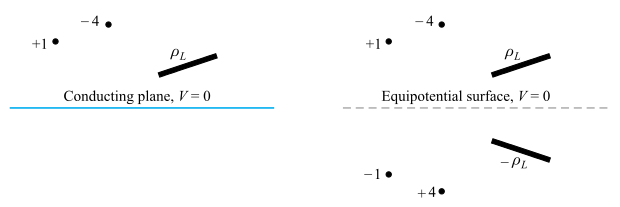
\includegraphics[scale=0.6]{image2.png}\\%Figure 16.17

C'est une sphère d'équation

\[x^2+y^2 + (z-2)^2 =8\] qui se trouve au-dessus du plan $xy$.

Le champ est le suivant
\begin{center}

\includegraphics[scale=0.7]{image4.png}\\
\end{center}
Le vecteur normal doit être pris comme $\hat{\vec N} = \zunit$.

On va prendre le disque qui forme la base de la sphère pour calculer l'intégrale. Son équation est $C : x^2 + y^2 = 4 $  et $S : x^2 + y^2 = 4 $ avec $S_2 \equiv 0 $.


Il faut d'abord calculer le rotationnel de manière générale et puis on pose $z\equiv 0$.

\includegraphics[scale=0.7]{image3.png}\\

\section{Théorème de la Divergence}
Ce théorème appartient à Gauss, Green et Ostrogradsky.

C'est un théorème réellement fondamental pour la suite. % Petit jeu de mots au calme

$S$ est une surface fermée orientée qui appartient à $\Re^3$.

\[\iiint_D \divt F \dif V = \oiint_S F \cdot N \dif S\]
C'est une relation qui fait le lien entre une intégrale de volume de et de surface.
\textit{
Cas particulier : 2D}

\begin{center}
\includegraphics[scale=0.5]{image5.png}\\

\end{center}

\[\iint _R \divt F \dif A = \oint _C F \cdot N \dif S\]
C'est un cas particulier du théorème de la divergence en 2D. On a pris une coupe d'un volume 3D.

\subsection{Interprétation de $\divt \vec F$}

On considère une sphère de $\Re ^3$ de rayon $\epsilon \to 0$ centrée en P.

Ce qui va rester pour l'intégrale triple, c'est
\[\divt F(P) \dfrac{4\pi}{3} \epsilon^3 = \oiint _{S_{\epsilon}} F \cdot N \dif S \]

On voit donc que

\[\divt F (P) =  \lim_{\epsilon \to 0 } \frac{1}{\dfrac{4\pi}{3} \epsilon^3} \oiint _{S_{\epsilon}} F \cdot N \dif S \]

C'est le flux/volume

\subsection{Application du théorème de divergence}

\subsubsection{Calcul d'un flux}
\[\vec F = x \xunit + y \yunit + z \zunit \]

Au CM4, nous avons calculé l'intégrale de flux à travers ce cylindre.

\includegraphics[scale=0.7]{image6.png}

On trouve donc

\[\iint_S F \cdot N \dif S = \iiint \divt f \dif V\]

On calcule donc

\[\divt F = \frac{\partial F_1}{\partial x}+ \frac{\partial F_2}{\partial y} + \frac{\partial F_3}{\partial z}= 1+1+1=3 = 3 \iiint \dif V = 6 \pi a^2 h\]

On avait obtenu la même chose au CM4, mais de façon légèrement plus compliquée.

\subsubsection{Calculer $\oiint_S(x^2+y^2)dS$ sur la sphère S de rayon $a$ centrée à l'origine}

\[x^2+y^2+z^2 = a^2\]

\begin{itemize}

\item Vérifions s'il s'agit d'une intégrale de flux.

On a $\hat N = \dfrac{1}{a} r $

Or le vecteur position vaut
\[r = x\xunit +y\yunit +z\zunit\]

On peut trouver
\[\dfrac{1}{a}r = \dfrac{1}{a}xi +\dfrac{1}{a}yj +\dfrac{1}{a}zk = \hat N\]

Il faut trouver F tel que $F\cdot \hat N = x^2 + y ^2 $

\[\Rightarrow F = ax\xunit +ay\yunit +0\zunit \]
\item Appliquer le théorème de la divergence

$$ I = \iiint_{Boule} \divt F \dif V = 2a \iiint_{Boule}\dif v$$

\[I = 2a \dfrac{4}{3}\pi a^3 = \dfrac{8}{3}\pi a^4\]
\end{itemize}

\begin{myrem}
Ne pas utiliser tel quel le théorème de la divergence si F n'est pas régulier dans D.


\emph{Exemple :} \[F = \dfrac{1}{\norm{r}^3} r \]

Non-régulier en $r=0$.

On établit un domaine $ D^* =D $ sans la boule centrée en 0 et puis on applique le théorème de la divergence à $D^*$.

Voir~\cite{adams2013calculus}, p.~910.
\end{myrem}

\begin{myrem}
\[\int_{C_{P_0 \to P_1}} \nabla f \cdot \dif r = f(P_1) - f(P_0) \]

\[\iint \rot F \cdot \dif S = \oint F \cdot \dif r \]

\[\iiint \divt F \dif V = \oiint_S F \cdot \dif S\]

Ces trois théorèmes sont des généralisations de :

\[\int_a^b \frac{\dif}{\dif x}f(x) \dif x = f(b) - f(a) \]

$\int$ (la dérivée de $f$) = $f$ évaluée aux bornes.
\end{myrem}
